% Compile with pdflatex + bibtex (e.g. upload the paper/ and figures/ folders to Overleaf).
\documentclass[11pt]{amsart}
\usepackage[margin=1.1in]{geometry}
\usepackage{amsmath,amssymb,amsthm}
\usepackage{graphicx}
\usepackage[colorlinks=true,linkcolor=blue!50!black,citecolor=blue!50!black,urlcolor=blue!50!black]{hyperref}
\usepackage{xcolor}
\usepackage{booktabs}

\graphicspath{{../figures/}}

\newtheorem{theorem}{Theorem}
\newtheorem{proposition}[theorem]{Proposition}
\newtheorem{lemma}[theorem]{Lemma}
\theoremstyle{remark}
\newtheorem{remark}[theorem]{Remark}

% Marks the parts that are still to be written. Remove before submission.
\newcommand{\todo}[1]{\par\noindent\fcolorbox{red!60!black}{red!5}{\parbox{\dimexpr\linewidth-2\fboxsep-2\fboxrule}{\small\textbf{TODO.} #1}}\par}

\title[Breaking the caustics of elliptic billiards]{From a gaokao ellipse to the onset of chaos:\\ how the caustics of elliptic billiards break}
\author{Boyan (Karina) Li}
\address{Department of Mathematics, University of California San Diego}
\email{TODO}
\date{\today}

\begin{abstract}
A billiard ball in an elliptical table never moves freely: every segment of its
path is tangent to one fixed confocal conic, and the product $d_1d_2$ of the
distances from the foci to the path is conserved. We give a self-contained,
elementary proof of these classical facts using only tools from high-school
analytic geometry, and verify them numerically to machine precision with a
simulator built on Vieta's formulas. We then deform the table
\todo{one sentence on the deformation family studied and the main result.}
\end{abstract}

\begin{document}
\maketitle

%======================================================================
\section{Introduction}

Problem 16 of the 2025 Chinese national college entrance examination
(National Paper~II) concerns the ellipse
\[
  C:\quad \frac{x^2}{4} + \frac{y^2}{2} = 1 .
\]
Students intersect a line with $C$, apply Vieta's formulas, and compute
chord lengths and areas. Exactly the same computation tells us where a
billiard ball moving inside $C$ hits the wall next
(Proposition~\ref{prop:next}). Iterating it turns a routine exam problem into a
dynamical system.

Billiards in an ellipse are \emph{integrable}: every orbit is confined to a
curve in phase space, labelled by a conserved quantity
(Figure~\ref{fig:phase}). A famous open problem, the \emph{Birkhoff
conjecture}~\cite{Birkhoff1927}, asserts that ellipses are the only
integrable convex billiard tables; see~\cite{AvilaDeSimoiKaloshin2016,
KaloshinSorrentino2018} for recent progress. This motivates our question:
\begin{quote}
\emph{When an elliptical table is deformed, how quickly does the conserved
quantity stop being conserved, and how does this relate to the onset of chaos?}
\end{quote}

\todo{State the contributions in 3--4 bullet points once Section~\ref{sec:deformed}
is done, and position them against the literature (Berry~\cite{Berry1981}
studied deformations of the circle; search for prior work on the
specific deformation family you choose).}

\paragraph{Outline.} Section~\ref{sec:ellipse} proves the classical results with
elementary tools. Section~\ref{sec:numerics} describes the simulator and
verifies Section~\ref{sec:ellipse} numerically. Section~\ref{sec:deformed}
studies deformed tables.

%======================================================================
\section{Billiards in an ellipse}\label{sec:ellipse}

Throughout, $C$ is the ellipse $x^2/a^2 + y^2/b^2 = 1$ with $a > b > 0$, foci
$F_{1,2} = (\mp c, 0)$ and $c^2 = a^2 - b^2$.

\subsection{The next bounce}

\begin{proposition}\label{prop:next}
Let $P = (x_0, y_0) \in C$ and $\mathbf d = (p, q) \ne \mathbf 0$ with
$\mathbf d \cdot \mathbf n \ne 0$, where $\mathbf n = (x_0/a^2,\, y_0/b^2)$.
The line $P + t\mathbf d$ meets $C$ again at $t = t^\ast$, where
\[
  t^\ast = -\,\frac{2\,(x_0p/a^2 + y_0q/b^2)}{p^2/a^2 + q^2/b^2}.
\]
\end{proposition}

\begin{proof}
Substituting $P + t\mathbf d$ into the equation of $C$ gives
$At^2 + Bt + C_0 = 0$ with $A = p^2/a^2 + q^2/b^2 > 0$,
$B = 2\,\mathbf d\cdot\mathbf n$, and $C_0 = x_0^2/a^2 + y_0^2/b^2 - 1 = 0$.
One root is $t = 0$, so by Vieta's formulas the other is $-B/A$.
\end{proof}

The vector $\mathbf n$ is an outward normal to $C$ at $P$. The law of
reflection then reads $\mathbf d' = \mathbf d - 2(\mathbf d\cdot\hat{\mathbf
n})\hat{\mathbf n}$, with $\hat{\mathbf n} = \mathbf n/|\mathbf n|$.

\subsection{Caustics}

\begin{theorem}[Caustic theorem]\label{thm:caustic}
Let $AB$ be a segment of a billiard orbit in $C$ that passes through neither
focus. If line $AB$ does not separate $F_1$ and $F_2$, every segment of the
orbit is tangent to one ellipse with foci $F_1, F_2$. If it does, every
segment is tangent to one hyperbola with foci $F_1, F_2$.
\end{theorem}

The proof uses three elementary tools: the optical property of the ellipse,
the shortest-path reflection trick, and congruent triangles.

\begin{lemma}[Optical property]\label{lem:optical}
At every $B \in C$ the normal line bisects $\angle F_1BF_2$.
\end{lemma}

\begin{remark}
In 2010 Anhui Problem~19 (paper type not confirmed), the ellipse through
$A(2,3)$ with foci on the $x$-axis and eccentricity $\tfrac12$ is
$x^2/16 + y^2/12 = 1$, and the bisector of $\angle F_1AF_2$ is
$2x - y - 1 = 0$. This is the normal line at $A$, as
Lemma~\ref{lem:optical} predicts.
\end{remark}

\begin{lemma}\label{lem:tangent}
Let $\ell$ be a line with $F_1, F_2$ strictly on one side and let $F_1'$ be
the reflection of $F_1$ in $\ell$. The ellipse with foci $F_1, F_2$ and major
axis $|F_1'F_2|$ is tangent to $\ell$ at $P_0 = F_1'F_2 \cap \ell$. If $\ell$
contains a chord $AB$ of $C$, then $P_0$ lies strictly between $A$ and $B$.
\end{lemma}

\begin{proof}
For $P \in \ell$, $|PF_1| + |PF_2| = |PF_1'| + |PF_2| \ge |F_1'F_2|$, with
equality only at $P_0$. So $\ell$ meets this ellipse only at $P_0$ and is
otherwise outside it, hence tangent. For the second claim, pick $X$ strictly
between $A$ and $B$. Then $|P_0F_1| + |P_0F_2| \le |XF_1| + |XF_2| < 2a$, so
$P_0$ is inside $C$.
\end{proof}

\begin{lemma}\label{lem:side}
If $A, B, C$ are consecutive bounce points, line $AB$ separates the foci if
and only if line $BC$ does.
\end{lemma}

\begin{proof}
Since the foci are inside $C$, line $AB$ separates them iff ray $BA$ lies
strictly inside $\angle F_1BF_2$. The reflection $\sigma_B$ in the normal at
$B$ maps this angle to itself and ray $BA$ to ray $BC$.
\end{proof}

\begin{figure}[t]
  \centering
  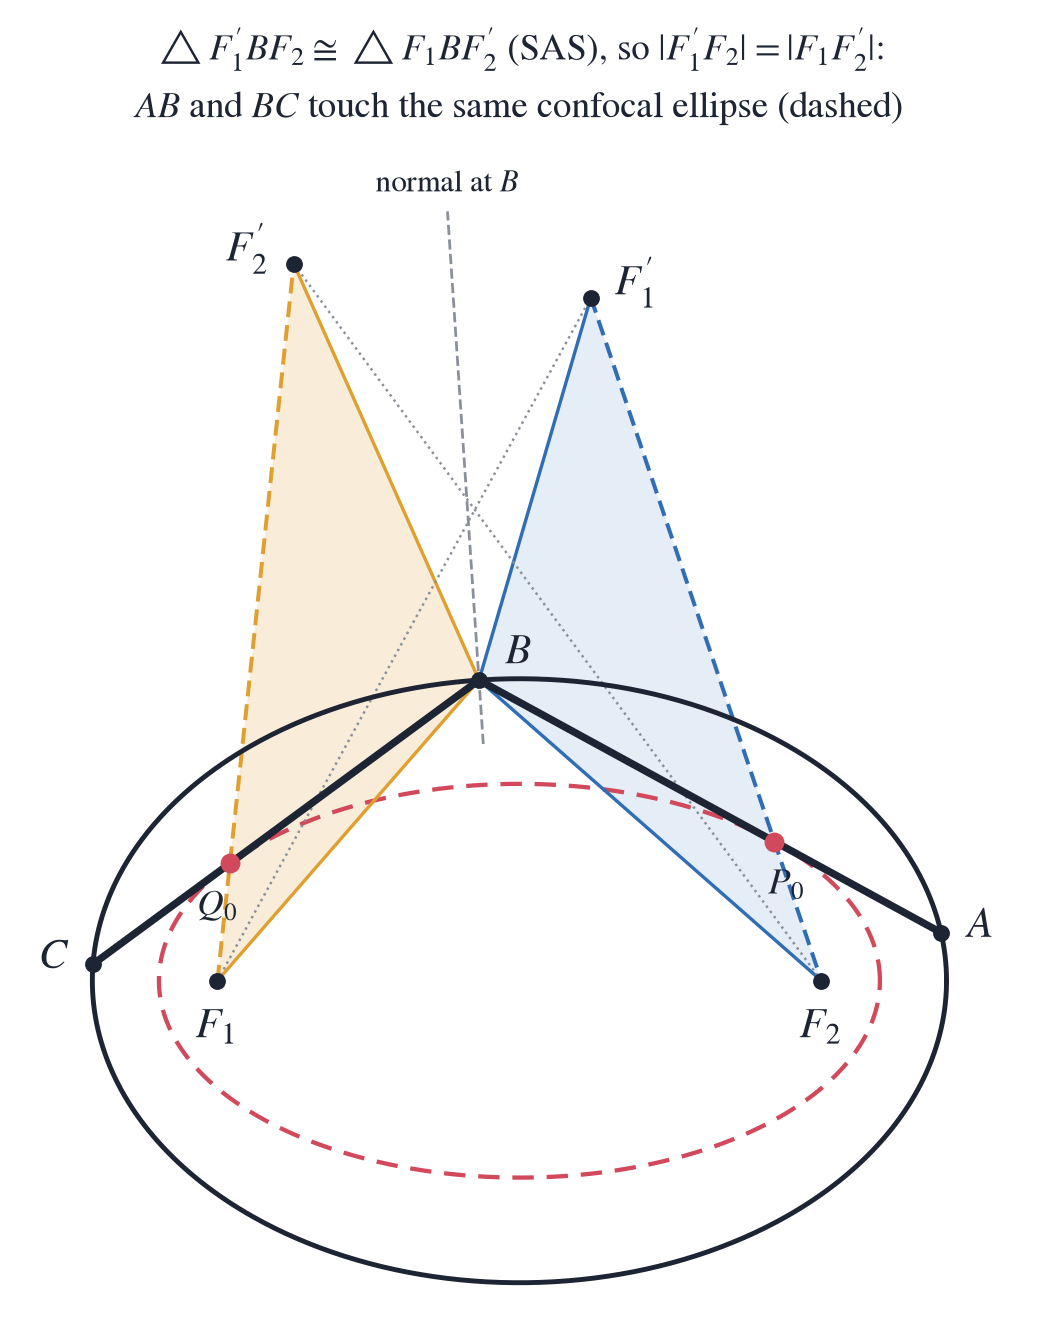
\includegraphics[width=0.62\linewidth]{proof.png}
  \caption{The construction in the proof of Theorem~\ref{thm:caustic}.}
  \label{fig:proof}
\end{figure}

\begin{proof}[Proof of Theorem~\ref{thm:caustic}, ellipse case]
Let $A, B, C$ be consecutive bounce points with line $AB$ not separating the
foci; by Lemma~\ref{lem:side}, neither does $BC$. Reflect $F_1$ in $AB$ to
$F_1'$ and $F_2$ in $BC$ to $F_2'$ (Figure~\ref{fig:proof}). By
Lemma~\ref{lem:tangent} it suffices to show $|F_1'F_2| = |F_1F_2'|$. We have
$|BF_1'| = |BF_1|$ and $|BF_2| = |BF_2'|$. By Lemma~\ref{lem:tangent}, ray $BA$
lies inside $\angle F_1'BF_2$ and ray $BC$ inside $\angle F_1BF_2'$, so
\[
  \angle F_1'BF_2 = \angle ABF_1 + \angle ABF_2, \qquad
  \angle F_1BF_2' = \angle CBF_1 + \angle CBF_2 .
\]
The reflection $\sigma_B$ swaps rays $BA \leftrightarrow BC$ (law of
reflection) and $BF_1 \leftrightarrow BF_2$ (Lemma~\ref{lem:optical}), so the
two right-hand sides are equal. By SAS,
$\triangle F_1'BF_2 \cong \triangle F_1BF_2'$.
\end{proof}

\todo{Hyperbola case of Theorem~\ref{thm:caustic} (replace the sum of focal
distances by the absolute difference).}

\subsection{The conserved quantity}

\begin{lemma}\label{lem:product}
The distances $d_1, d_2$ from the foci to any tangent line of $C$ satisfy
$d_1d_2 = b^2$.
\end{lemma}

\begin{proof}
See \texttt{notes/03-conserved-quantity.md}.
\todo{Write out the proof here.}
\end{proof}

\begin{theorem}\label{thm:conserved}
Write the confocal family as $\mathcal C_\lambda: x^2/(a^2-\lambda) +
y^2/(b^2-\lambda) = 1$. Along any non-focal orbit with caustic
$\mathcal C_\lambda$, the signed product of the focal distances to each
segment equals $b^2 - \lambda$. In particular, it is conserved.
\end{theorem}

\todo{Proof, from Theorem~\ref{thm:caustic} and Lemma~\ref{lem:product}
(plus its hyperbola version).}

\subsection{Poncelet's porism}

If one orbit with caustic $\mathcal C_\lambda$ closes after $n$ bounces, then
every orbit with that caustic closes after $n$ bounces, and all of them have
the same perimeter~\cite{Poncelet1822, DragovicRadnovic2011, Tabachnikov2005}.
Figure~\ref{fig:poncelet} illustrates this.

%======================================================================
\section{Numerical method and verification}\label{sec:numerics}

The simulator iterates Proposition~\ref{prop:next} and the reflection law.
After each bounce the new point is rescaled radially onto $C$ to prevent
round-off drift. Every claim of Section~\ref{sec:ellipse} is checked
numerically by \texttt{verify.py}; Table~\ref{tab:checks} summarizes the
results.

\begin{table}[h]
\centering
\begin{tabular}{lr}
\toprule
Check (on $x^2/4 + y^2/2 = 1$) & max.\ error \\
\midrule
Each step of the proof of Thm.~\ref{thm:caustic}, 300 random orbits & $7\times10^{-14}$ \\
$d_1d_2$ constant, 5000 bounces (ellipse / hyperbola caustic) & $1.9\times10^{-13}$ \\
Each segment tangent to $\mathcal C_{b^2 - d_1d_2}$ & $1.9\times10^{-13}$ \\
Poncelet closure, rotation numbers $1/5, 1/4, 2/7, 1/3$ & $2.2\times10^{-13}$ \\
Equal perimeters, same rotation numbers & $1.4\times10^{-13}$ \\
Perimeter for rotation number $1/4$ equals $4\sqrt{a^2+b^2}$ & $2.5\times10^{-14}$ \\
\bottomrule
\end{tabular}
\caption{Numerical verification of Section~\ref{sec:ellipse}.}
\label{tab:checks}
\end{table}

\begin{figure}[t]
  \centering
  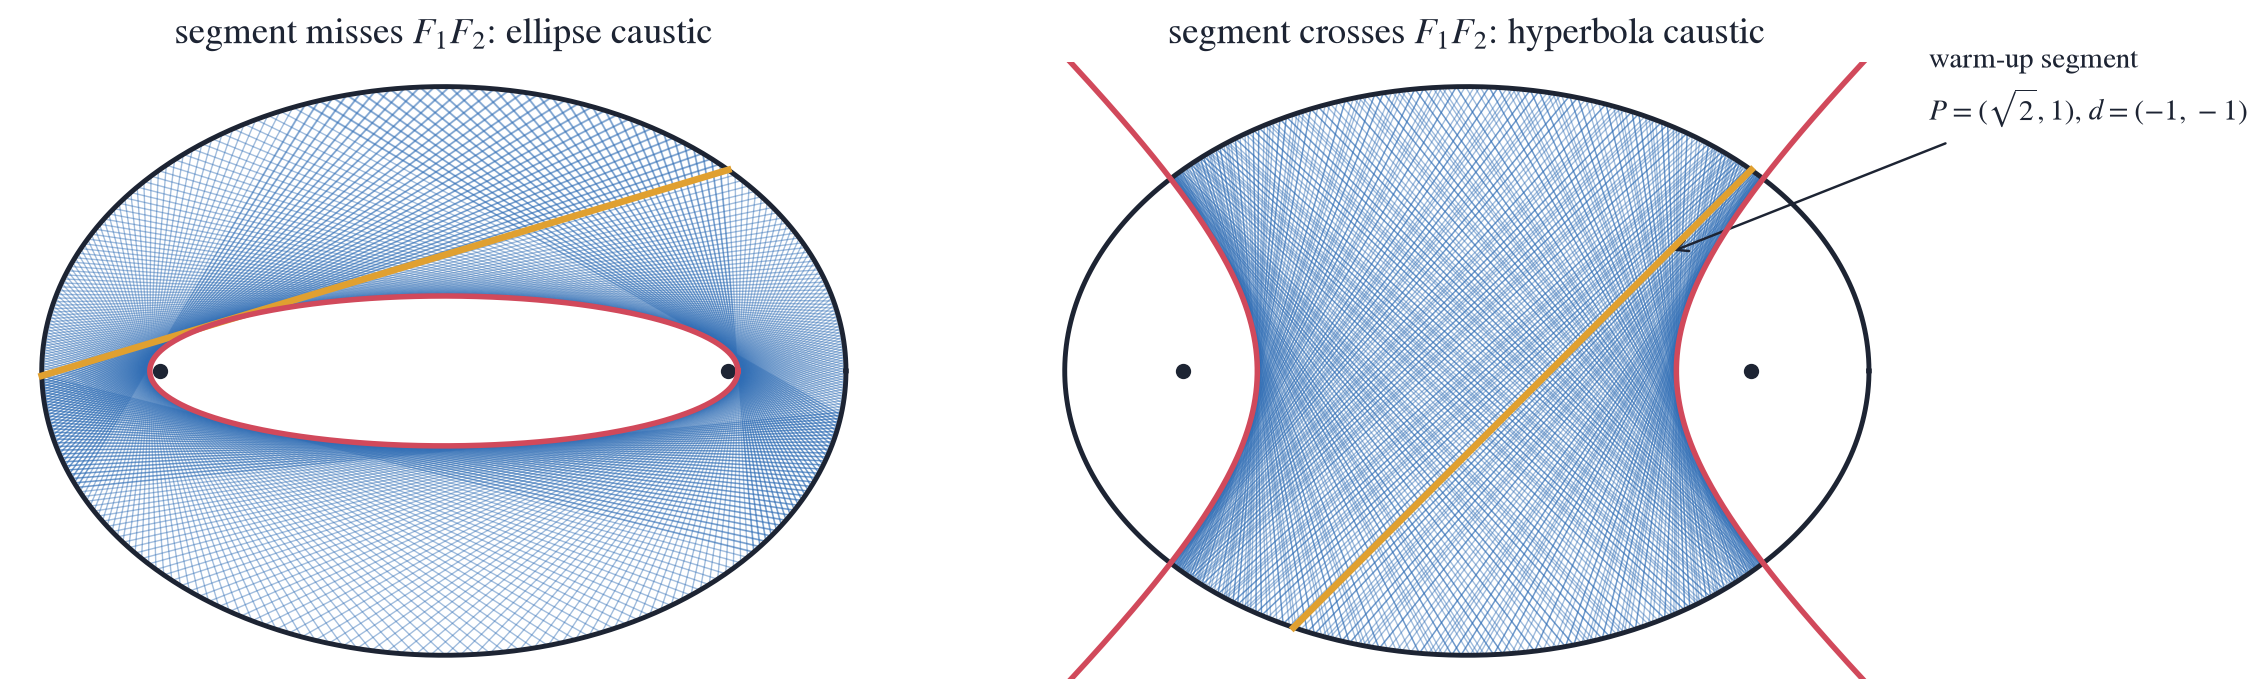
\includegraphics[width=\linewidth]{caustics.png}
  \caption{Left: an orbit with an ellipse caustic. Right: the orbit of the
  warm-up problem ($P = (\sqrt2, 1)$, $\mathbf d = (-1,-1)$) crosses the focal
  segment, so its caustic is a hyperbola.}
  \label{fig:caustics}
\end{figure}

\begin{figure}[t]
  \centering
  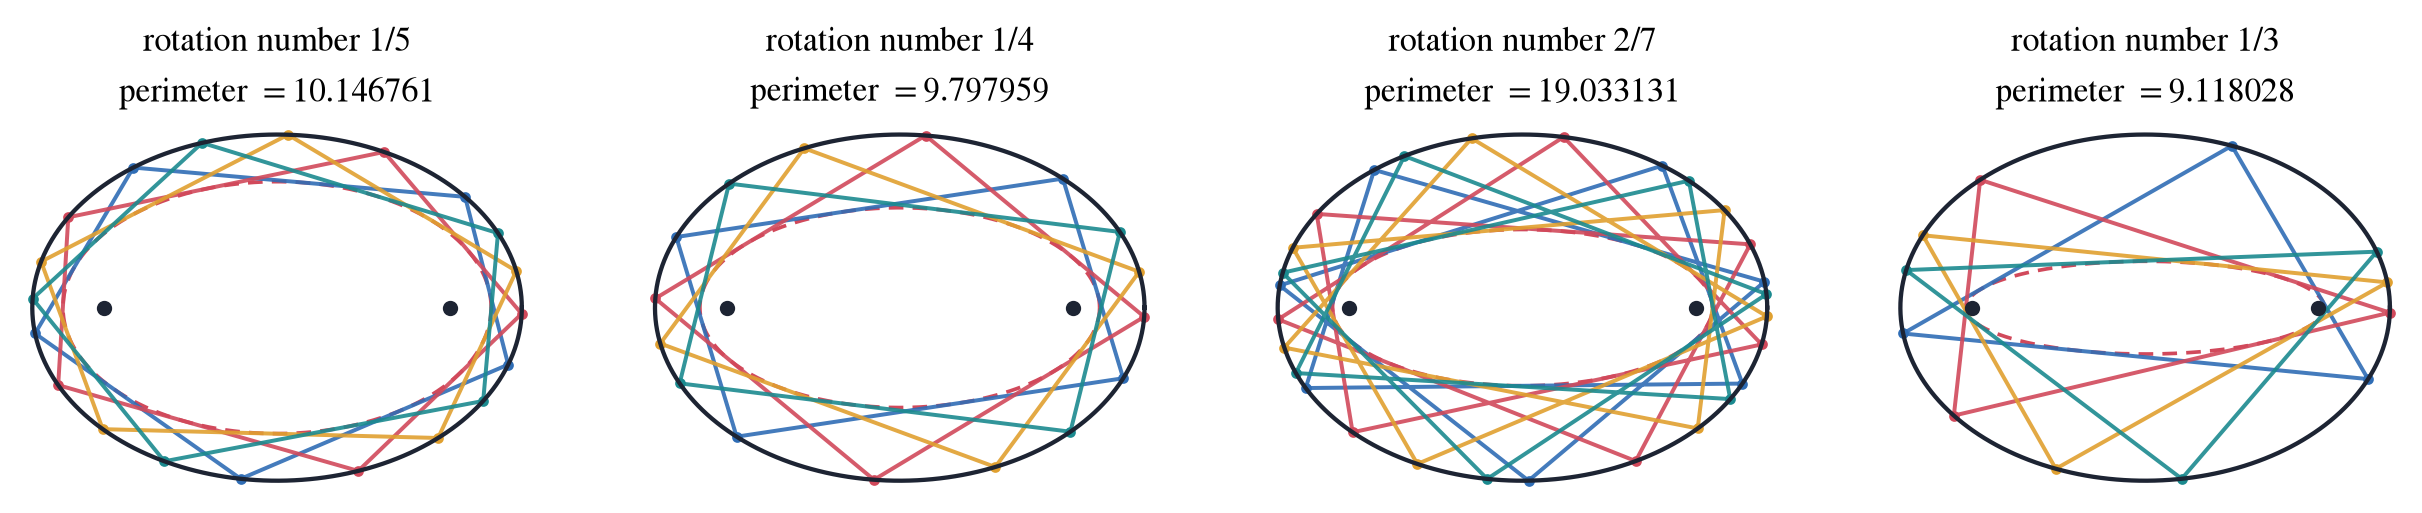
\includegraphics[width=\linewidth]{poncelet.png}
  \caption{Poncelet's porism: four orbits for each rotation number, all closing
  with equal perimeters.}
  \label{fig:poncelet}
\end{figure}

\begin{figure}[t]
  \centering
  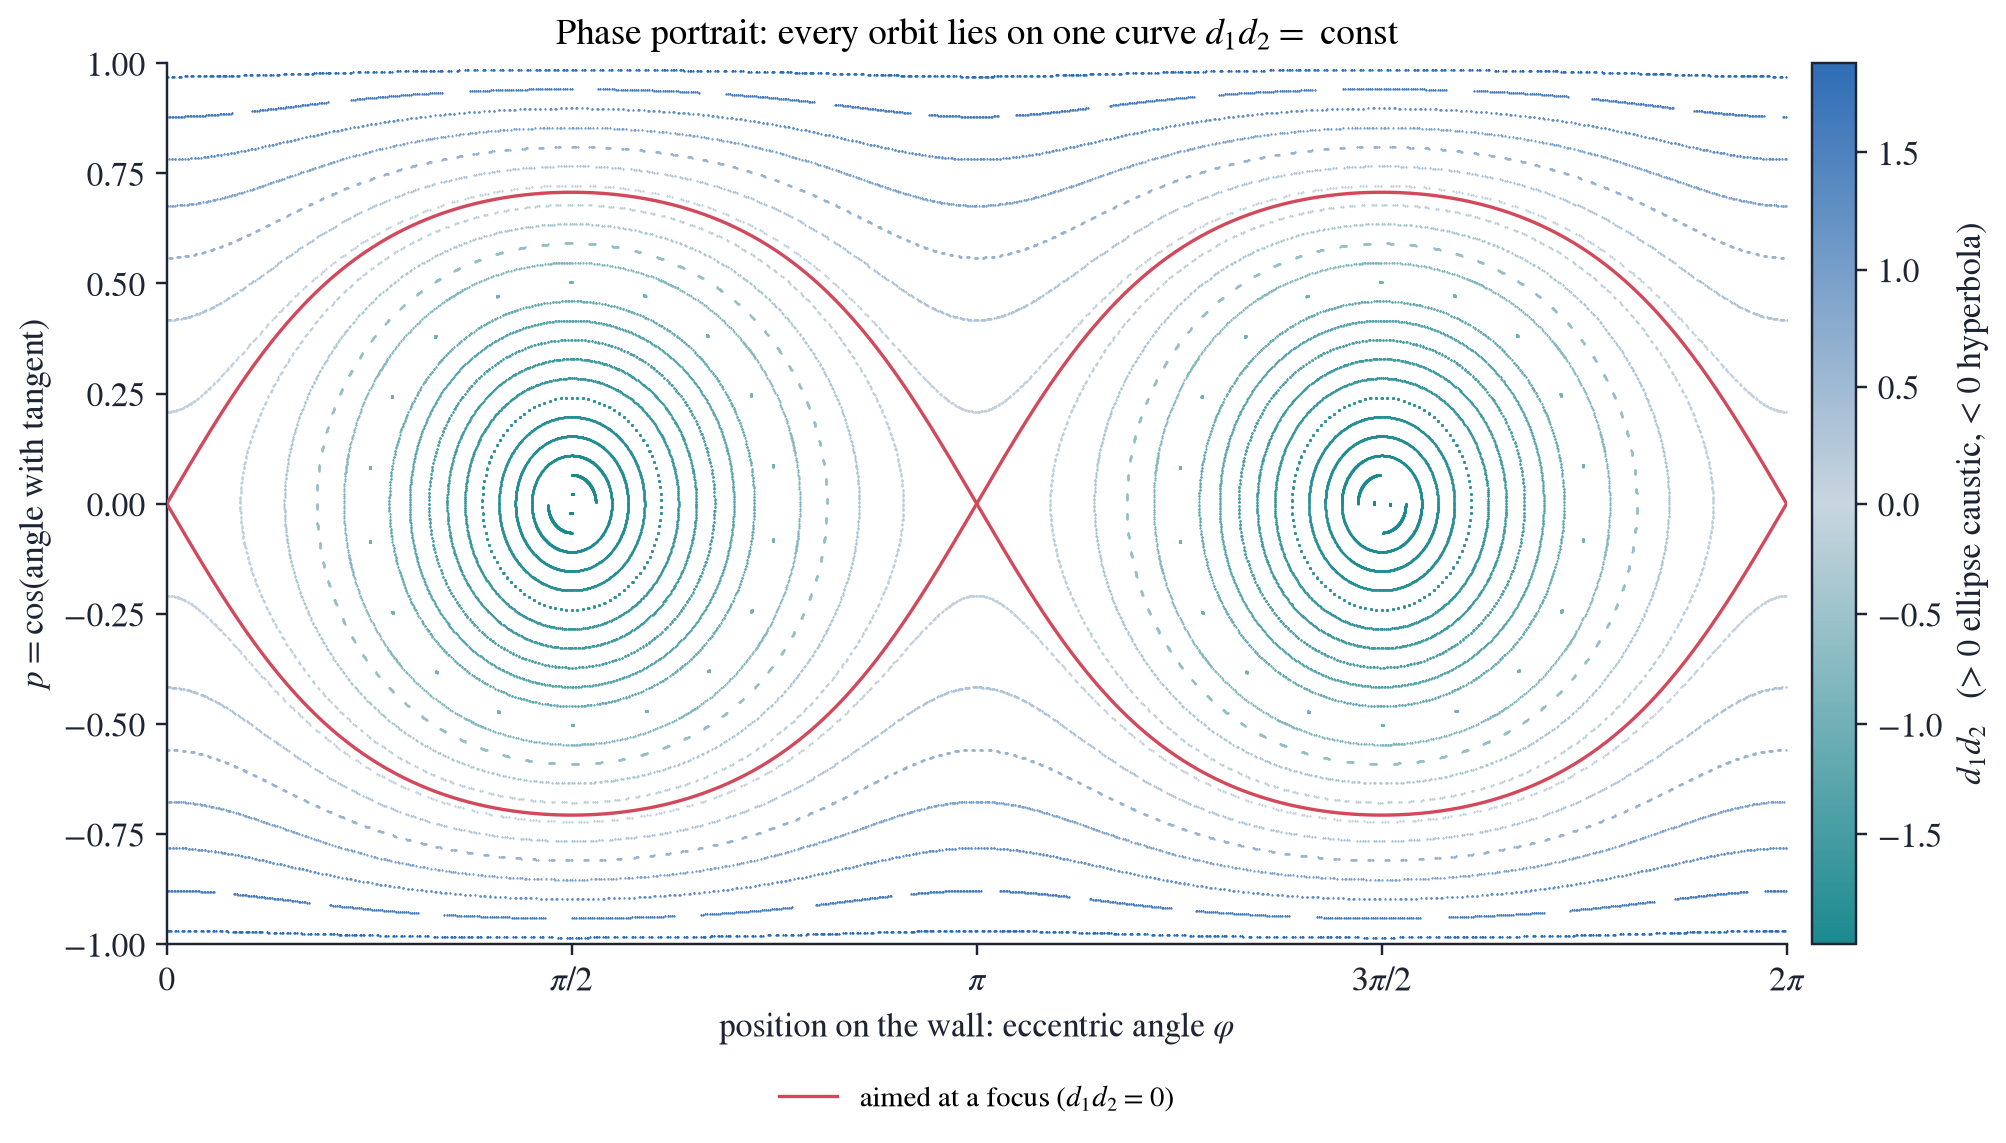
\includegraphics[width=\linewidth]{phase.png}
  \caption{Phase portrait of the elliptic billiard. Each orbit lies on a level
  curve of $d_1d_2$. The red curves ($d_1d_2 = 0$) separate the ellipse-caustic
  and hyperbola-caustic regions.}
  \label{fig:phase}
\end{figure}

%======================================================================
\section{Deformed tables}\label{sec:deformed}

\todo{This section is the original contribution and is to be written by the
author. Suggested structure:
(1) the deformation family, e.g.\ superellipses $|x/a|^p + |y/b|^p = 1$ with
$p$ near $2$, or the stadium;
(2) how the next bounce is computed when Vieta's formula is no longer
available (root finding);
(3) phase portraits as $p$ moves away from $2$, showing which invariant
curves survive (KAM, Lazutkin~\cite{Lazutkin1973}) and where chaotic layers
appear;
(4) a quantitative measure of how $d_1d_2$ fails to be conserved, as a
function of the deformation;
(5) Lyapunov exponents, compared with the stadium~\cite{Bunimovich1979}.}

%======================================================================
\section{Discussion}

\todo{What the results say about the question in the introduction, their
limitations, and open questions.}

\section*{Acknowledgements and use of AI}

\todo{Disclose AI assistance precisely, following the target journal's policy.
See \texttt{LOG.md} for the record of which parts were drafted with AI help.}

\bibliographystyle{amsplain}
\bibliography{refs}

\end{document}
